\chapter{Countermeasures}
\label{countermeasures}
In this chapter, we describe the various activities that the operator can put in place to strengthen the traffic of a LoRaWAN network, decreasing the number of exposed ED recognized by PIVOT. The final objective of the administrator is to modify the devices' parameters to avoid being detected again by our system. In other words, it has to reduce the overall detection curve of PIVOT.

\vspace{5mm} %5mm vertical space

% dummy packets don't work
The LoRa network topology is strongly constrained. Not allowing direct sensor-to-sensor communication, a strategy could be to obfuscate the traffic by adding dummy packets to EDs transmissions. Since each LoRa packet payload is encrypted, dummy packets are indistinguishable from those containing information allowing only the application server to filter them. To the detriment of its effectiveness, this mechanism impacts performance and costs. Firstly, the transmission of additional packets requires more energy, reducing the lifetime of the ED. Secondly, it also reduces channel availability.

\vspace{5mm}

In this work, rather than altering traffic by adding new data to the network, we propose to change the flow generated by the vulnerable devices, hiding their periodic behaviors. There are two possible strategies, of which we will analyze the advantages and disadvantages.
\\
The first method regularizes the flow by requiring endpoints to send packets following the same frequencies (for example, each hour). Although it may prove to be an effective method, it is not practical for all applications, especially those that require real-time response.
\begin{figure}[H]
    \centering
    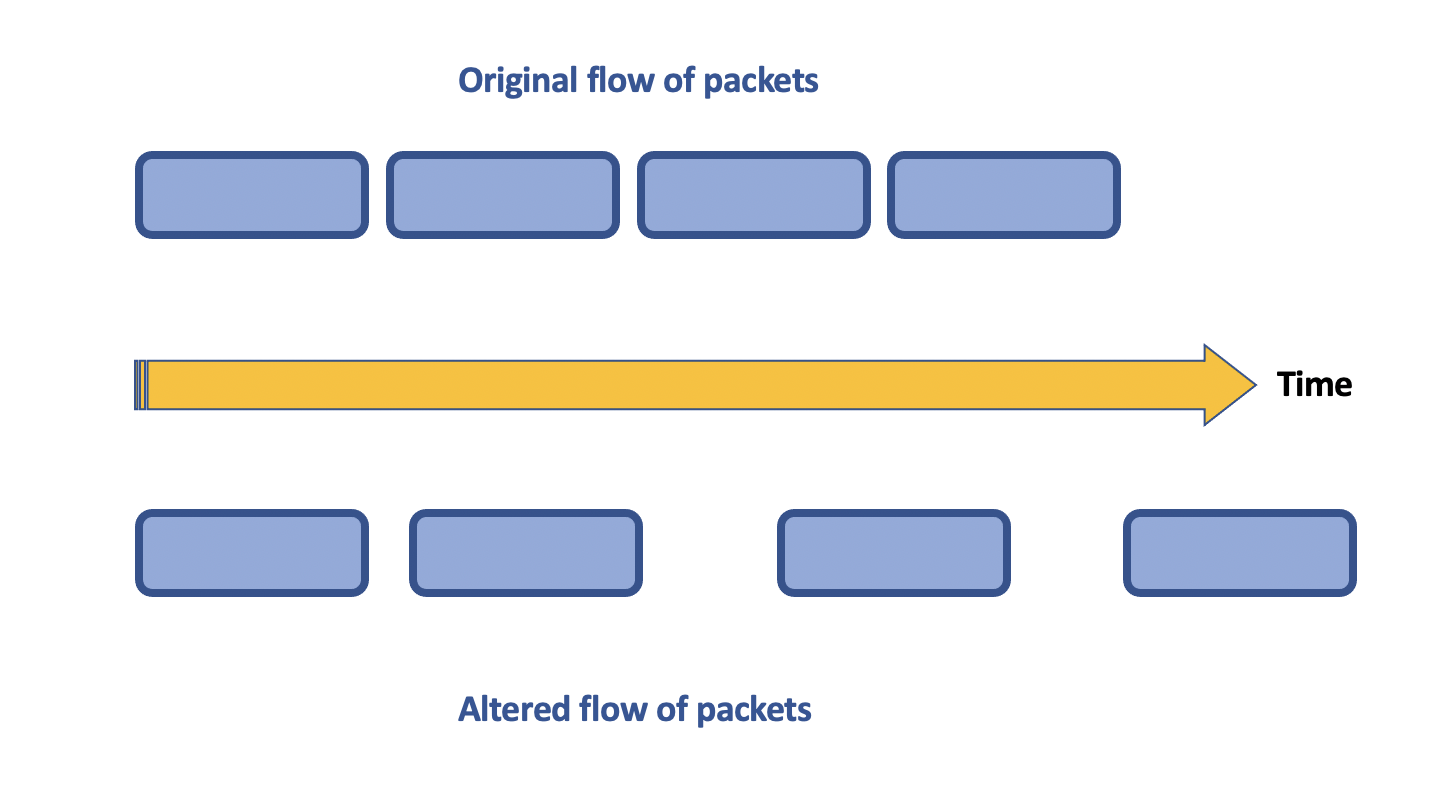
\includegraphics[width=0.7\linewidth]{images/countermeasures/flow.png}
    \caption{The altered flow}
    \label{fig:flow}
\end{figure}
We can add a random delay to the non-protected traffic. When the delay is high enough, it hides the correlation between a device and its pattern. The required delay can be extracted from a \textit{pseudo-random} number sampling, a procedure for generating numbers distributed according to a given \textit{probability distribution}. A well know pseudo-random number sampling method is the inverse transform sampling, which produces instances using the Cumulative Distribution Function (CDF) \(\ F_{X} \) of the random variable \(\ X \). The function \(\ F_{X} \) takes as input some value \(\ x \) outputs the probability of obtaining \(\ X \leq x \). 
\[\ F_{X}(x) = P(X \leq x) = p \]
The inverse transform sampling uses the inverse of CFD. The \(\ F_{X}^{-1} \) takes \(\ p \) as input and returns \(\ x \), where \(\ p \) is uniformly distributed. With this method, we can sample from any \(\ F_{X} \) if \(\ F_{X}^{-1}  \) is known. We need just to take values \(\ u \sim U(0,1) \) and then, through \(\ F_{X}^{-1}  \), obtain \(\ x \)'s.
\[\ F_{X}^{-1}(u) = x \]

\subsubsection{The exponential distribution}
Our idea is to simulate a random variable \(\ X \) that follows the \textit{exponential} distribution with mean \(\ \lambda \) i.e. \(\ X \sim Exp(\lambda) \). In queing theory, this distribution lends itself well to modeling customer interarrival times or service times for several reasons \cite{QUEUING_THEORY}. First, the exponential function is a strictly decreasing function of \(\ t \), meaning that after an arrival has occurred, the amount of waiting time until the next arrival is more likely to be small than large. Second, the exponential distribution is memoryless. This property implies that the time until the next arrival don't depend the time that has already passed. Finally, the exponential distribution is striclty correlated to the Poisson distribution.
\begin{figure}[H]
    \centering
    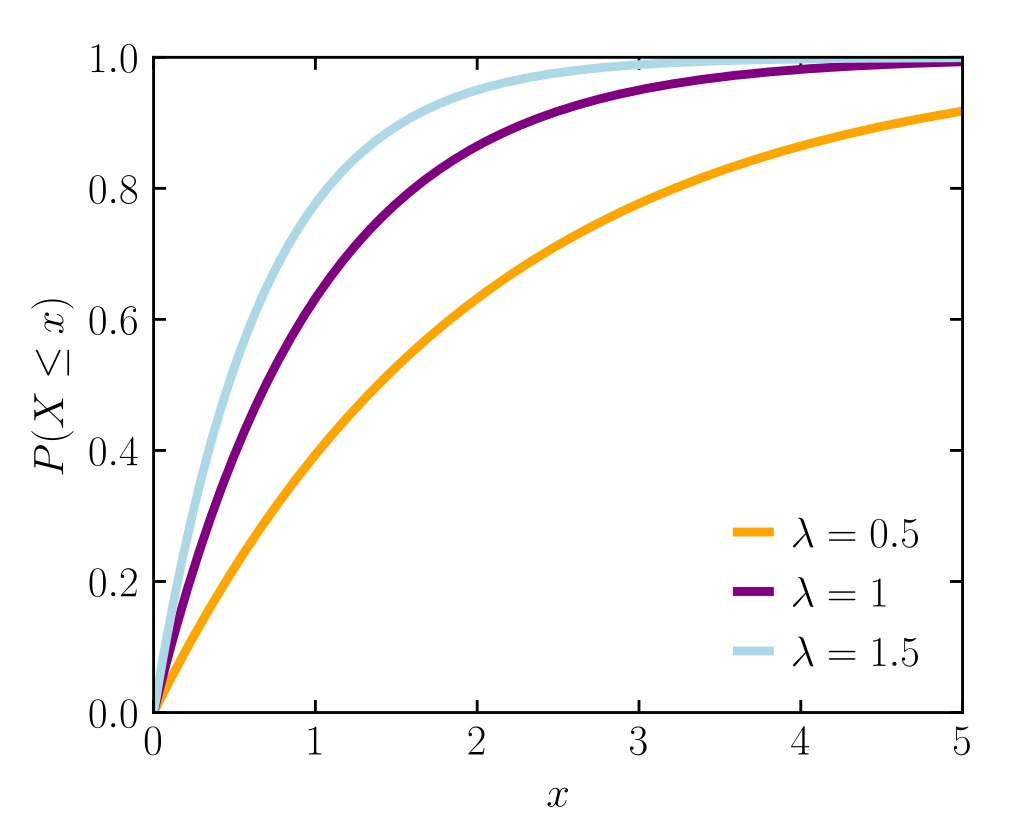
\includegraphics[width=0.7\linewidth]{images/countermeasures/cumulative_distribution_function.png}
    \caption{CDF of the exponential distribution}
    \label{fig:cdf}
\end{figure}
Going into the details, the Probability Density Function (PDF) of the exponential distribution is:
\[\ f(x, \lambda ) = \lambda e^{-\lambda x}, x \geq 0, \lambda \geq 0 \]
while the Cumulative Distribution Function (CDF), shown in Figure \ref{fig:cdf} is defined as follows:
\[\ F(x) = 1 - e^{-\lambda x} \]
By solving \(\ p = F(x) \), we obtain the inverse function
\[\ x = F^{-1}(p) = -\frac{1}{\lambda}\ln(1-p) \]
The idea is illustrated in Figure \ref{fig:distribution}. Random numbers are generated from a uniform distribution between \(\ 0 \) and \(\ 1 \). Each of the points is mapped according to \(\ x = F_{-1}(y) \). We can observe that using this strategy, most of the points end up close to 0, while only a few of them end up having high values.
\begin{figure}[H]
    \centering
    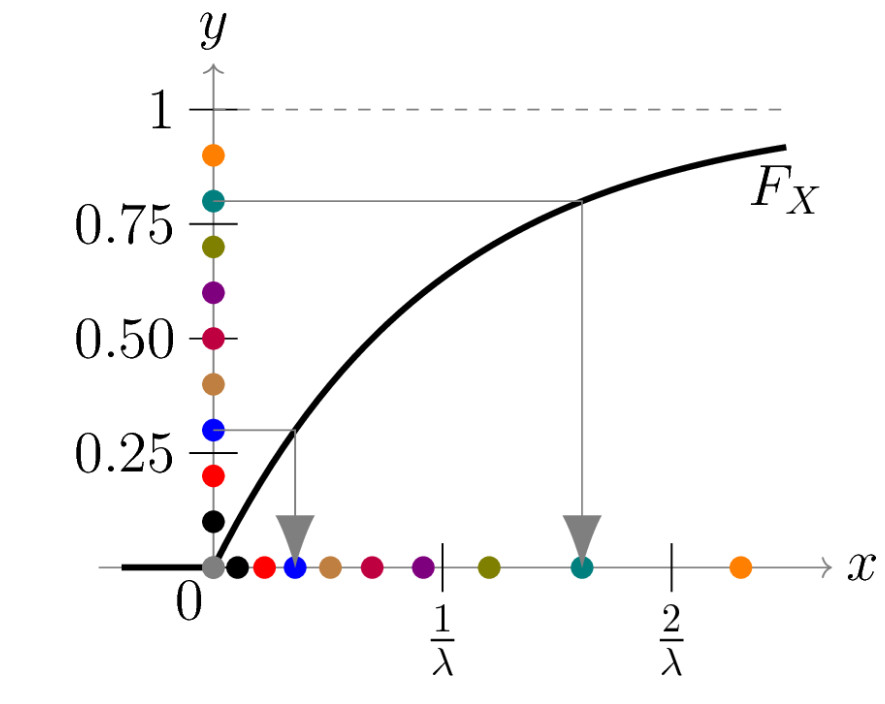
\includegraphics[width=0.7\linewidth]{images/countermeasures/inverse_transformation_method_for_exponential_distribution.jpg}
    \caption{Inverse transformation method for exponential distribution}
    \label{fig:distribution}
\end{figure}

%The choice of the delay cannot be completely random. EDs can occupy the channel for a limited portion of time, called  \textit{duty cycle}. It is commonly set to 1\%, or 1-time unit every 100-time units \cite{8030482}.
\begin{figure}[H]
    \centering
    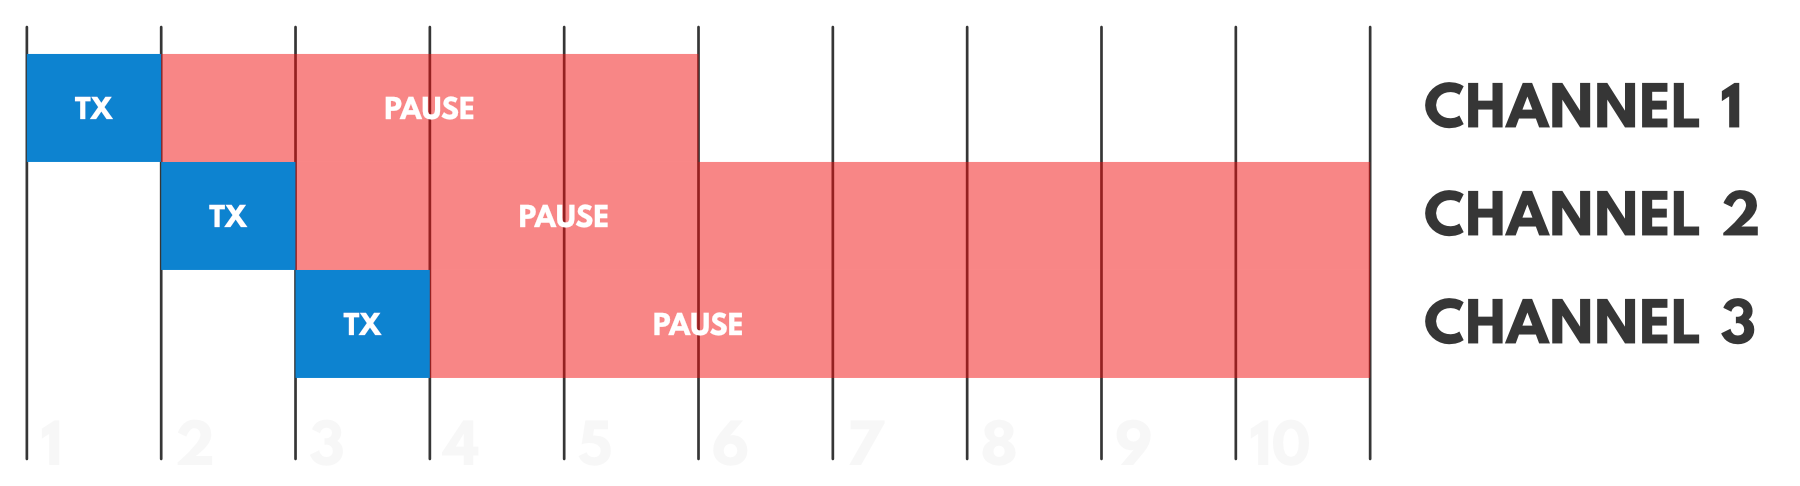
\includegraphics[width=0.7\linewidth]{images/countermeasures/duty_cycle.png}
    \caption{The duty cycle of LoRaWAN}
    \label{fig:duty_cycle}
\end{figure}